\chapter{PENGUJIAN DAN ANALISIS}
\label{chap:pengujiananalisis}

% Ubah bagian-bagian berikut dengan isi dari pengujian dan analisis

Pada bab ini akan membahas tentang pengujian sistem perencanaan gerakan mobil otonom dengan menggunakan algoritma DQN. Kemudian, akan dilakukan analisis terhadap hasil simulasi sistem
perencanaan gerakan mobil otonom yang telah dirancang.

\section{Training DQN}
\label{sec:training_dqn}
Training algoritma DQN dilakukan dengan menggunakan hardware berikut:
\begin{table}[H]
	\begin{tabular}{ll}
		\textbf{CPU}  & Intel Core i5              \\
		\textbf{GPU}  & Nvidia GTX 1060 - 6GB VRAM \\
		\textbf{RAM}  & 8GB                        \\
		\textbf{Disk} & 256GB SSD M.2              \\
		\textbf{OS}   & Windows 10                
	\end{tabular}
\caption{Hardware yang digunakan untuk learning.}
\label{tb:hardwaresetup}
\end{table}

Learning dilakukan dengan mesin lokal menggunakan GPU. Lingkungan software machine learning yang digunakan pada learning berupa:

\begin{table}[H]
	\begin{tabular}{ll}
		\textbf{Software}  & \textbf{Version}              \\
		tensorflow-gpu  & 1.13.1	\\
		keras  & 2.2.5					\\
		h5py & 3.1              \\
		python & 3.7.9              \\
	\end{tabular}
	\caption{Lingkungan software yang digunakan untuk learning.}
	\label{tb:softwaresetup}
\end{table}


Hasil dari proses training tersebut adalah model jaringan DQN yang merepresentasikan sistem perencanaan gerakan mobil otonom. Model tersebut disimpan dalam sebuah file berformat .model yang
selanjutnya dapat divisualisasikan dengan tensorboard untuk melihat hasil training algoritma DQN.

\subsection{Training DQN pada Bundaran Simpang Empat dengan Segmentasi Grayscale}
\label{sec:training_dqn_bundaran_simpangempat_segmentasi_grayscale}

\begin{figure}[H] 
	\centering
	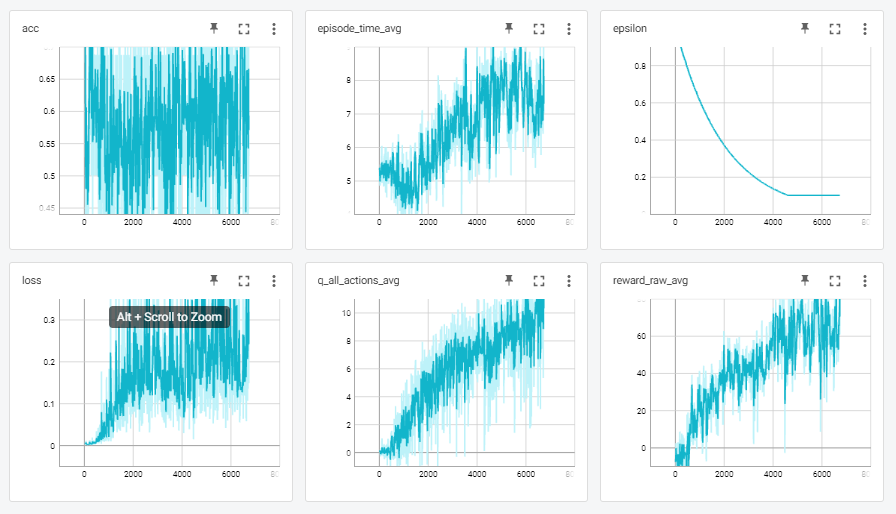
\includegraphics[width=1\linewidth]{images/tensorboard_bundaran_simpangempat_segmentasi_grayscale}
	\caption{Tensorboard pada Bundaran Simpang Empat dengan Segmentasi Grayscale}
	\label{fig:tensorboard_bundaran_simpangempat_segmentasi_grayscale}
\end{figure}

Dari hasil visualisasi training DQN pada Gambar \ref{fig:tensorboard_bundaran_simpangempat_segmentasi_grayscale}, dapat dilihat bahwa proses training algoritma DQN telah berjalan dengan baik. Hal itu dapat dilihat dari nilai akurasi, episode time, dan reward berkendara mobil otonom yang mengalami tren kenaikan seiring dengan berjalannya proses training.

\subsection{Training DQN pada Bundaran Simpang Empat dengan Segmentasi Lanjutan}
\label{sec:training_dqn_bundaran_simpangempat_segmentasi_hitam_putih}

\subsection{Training DQN pada Bundaran Tanpa Simpang dengan Segmentasi Lanjutan}
\label{sec:training_dqn_bundaran_nosimpang_segmentasi_hitam_putih}

\iffalse
Training algoritma DQN dengan
berlangsung selama 81 jam, 12 menit, dan 38 detik. Berikut adalah hasil visualisasi training algoritma DQN:

\begin{figure}[H] 
	\centering
	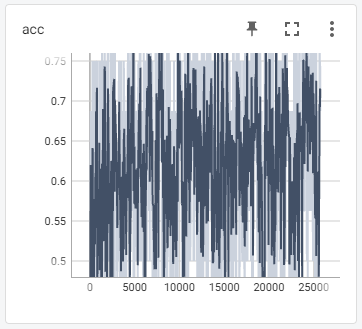
\includegraphics[width=.7\linewidth]{images/acc}
	\caption{Nilai akurasi}
	\label{fig:acc}
\end{figure}
\begin{figure}[H] 
	\centering
	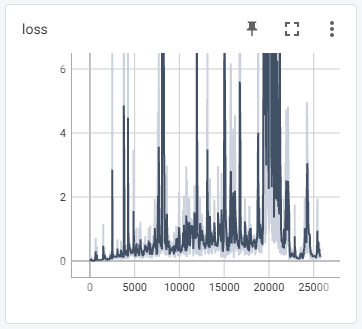
\includegraphics[width=.7\linewidth]{images/loss}
	\caption{Nilai loss}
	\label{fig:loss}
\end{figure}
\begin{figure}[H] 
	\centering
	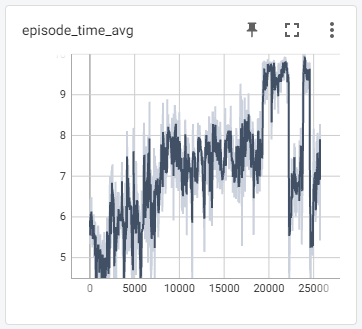
\includegraphics[width=.7\linewidth]{images/episode_time_avg}
	\caption{Rerata waktu episode}
	\label{fig:episode_time_avg}
\end{figure}
\begin{figure}[H] 
	\centering
	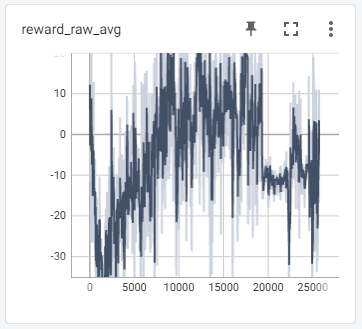
\includegraphics[width=.7\linewidth]{images/reward_raw_avg}
	\caption{Rerata nilai reward \textit{raw}}
	\label{fig:reward_raw_avg}
\end{figure}
\begin{figure}[H] 
	\centering
	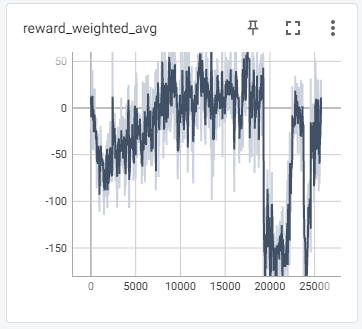
\includegraphics[width=.7\linewidth]{images/reward_weighted_avg}
	\caption{Rerata nilai reward \textit{weighted}}
	\label{fig:reward_weighted_avg}
\end{figure}
\begin{figure}[H] 
	\centering
	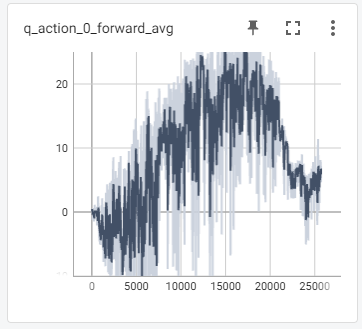
\includegraphics[width=.7\linewidth]{images/q_action_0_forward_avg}
	\caption{Nilai rerata q dari action forward}
	\label{fig:q_action_0_forward_avg}
\end{figure}
\begin{figure}[H] 
	\centering
	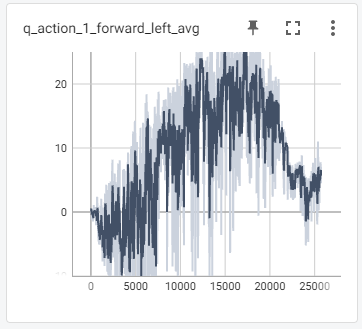
\includegraphics[width=.7\linewidth]{images/q_action_1_forward_left_avg}
	\caption{Nilai rerata q dari action forward left}
	\label{fig:q_action_1_forward_left_avg}
\end{figure}
\begin{figure}[H] 
	\centering
	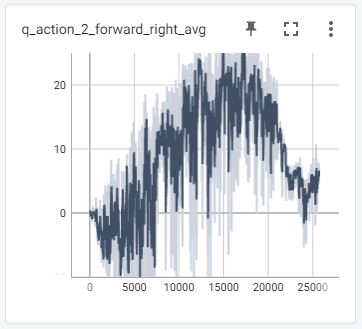
\includegraphics[width=.7\linewidth]{images/q_action_2_forward_right_avg}
	\caption{Nilai rerata q dari action forward right}
	\label{fig:q_action_2_forward_right_avg}
\end{figure}
\begin{figure}[H] 
	\centering
	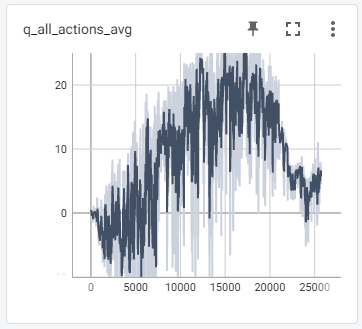
\includegraphics[width=.7\linewidth]{images/q_all_actions_avg}
	\caption{Nilai rerata q dari seluruh action}
	\label{fig:q_all_actions_avg}
\end{figure}

Dari hasil visualisasi training DQN diatas, dapat dilihat bahwa proses training algoritma DQN telah berjalan dengan baik. Hal itu dapat dilihat dari nilai akurasi, \textit{episode time}, dan \textit{reward} berkendara mobil otonom yang mengalami tren kenaikan seiring dengan berjalannya proses training.

\fi

\section{Pengujian Model DQN}
\label{sec:pengujian_model_dqn}

Pada bagian ini, akan dilakukan pengujian model hasil dari proses training DQN. Pengujian dilakukan saat lingkungan berkendara dalam kondisi normal.

\subsection{Pengujian Model DQN pada Bundaran Simpang Empat dengan Segmentasi Grayscale}
\label{sec:pengujian_dqn_bundaran_simpangempat_segmentasi_grayscale}

Setelah dilakukan tiga kali pengujian, didapatkan hasil seperti berikut:

% Please add the following required packages to your document preamble:
% \usepackage{graphicx}
\begin{table}[H]
	\resizebox{\columnwidth}{!}{%
		\begin{tabular}{|l|l|l|l|l|}
			\hline
			episode\_time & speed\_avg & angle\_deviation\_avg & distance\_deviation\_avg & reward\_avg \\ \hline
			24            & 40.2       & 17.3                  & 2.0                      & 0.32        \\ \hline
			25            & 40.1       & 20.8                  & 1.7                      & 0.28        \\ \hline
			16            & 38.8       & 16.6                  & 1.8                      & 0.32        \\ \hline
		\end{tabular}%
	}
	\caption{Hasil pengujian.}
	\label{tb:hasilpengujian}
\end{table}


\subsection{Pengujian Model DQN pada Bundaran Simpang Empat dengan Segmentasi Lanjutan}
\label{sec:pengujian_dqn_bundaran_simpangempat_segmentasi_hitam_putih}

\subsection{Pengujian Model DQN pada Bundaran Tanpa Simpang dengan Segmentasi Lanjutan}
\label{sec:pengujian_dqn_bundaran_nosimpang_segmentasi_hitam_putih}


\iffalse
\subsection{Hasil Setelah Learning 12 jam}
\label{sec:hasil_learning_12}
Setelah learning selama 12 jam, didapatkan model reinforcement yang sudah cukup memahami kehadiran bundaran di depan agent. Pada salah satu run simulasi Gambar \ref{fig:uji0}, didapatkan agent yang mampu bergerak lurus ke depan hingga mendekati bundaran, dan mampu melakukan manuver kanan lalu ke kiri lagi (dan arah kembali sejajar dengan arah pada saat start) agar tidak menyentuh bundaran. Meskipun pada akhirnya agent menyentuh object rumah pada ujung jalan.

\begin{figure}[H] 
	\centering
	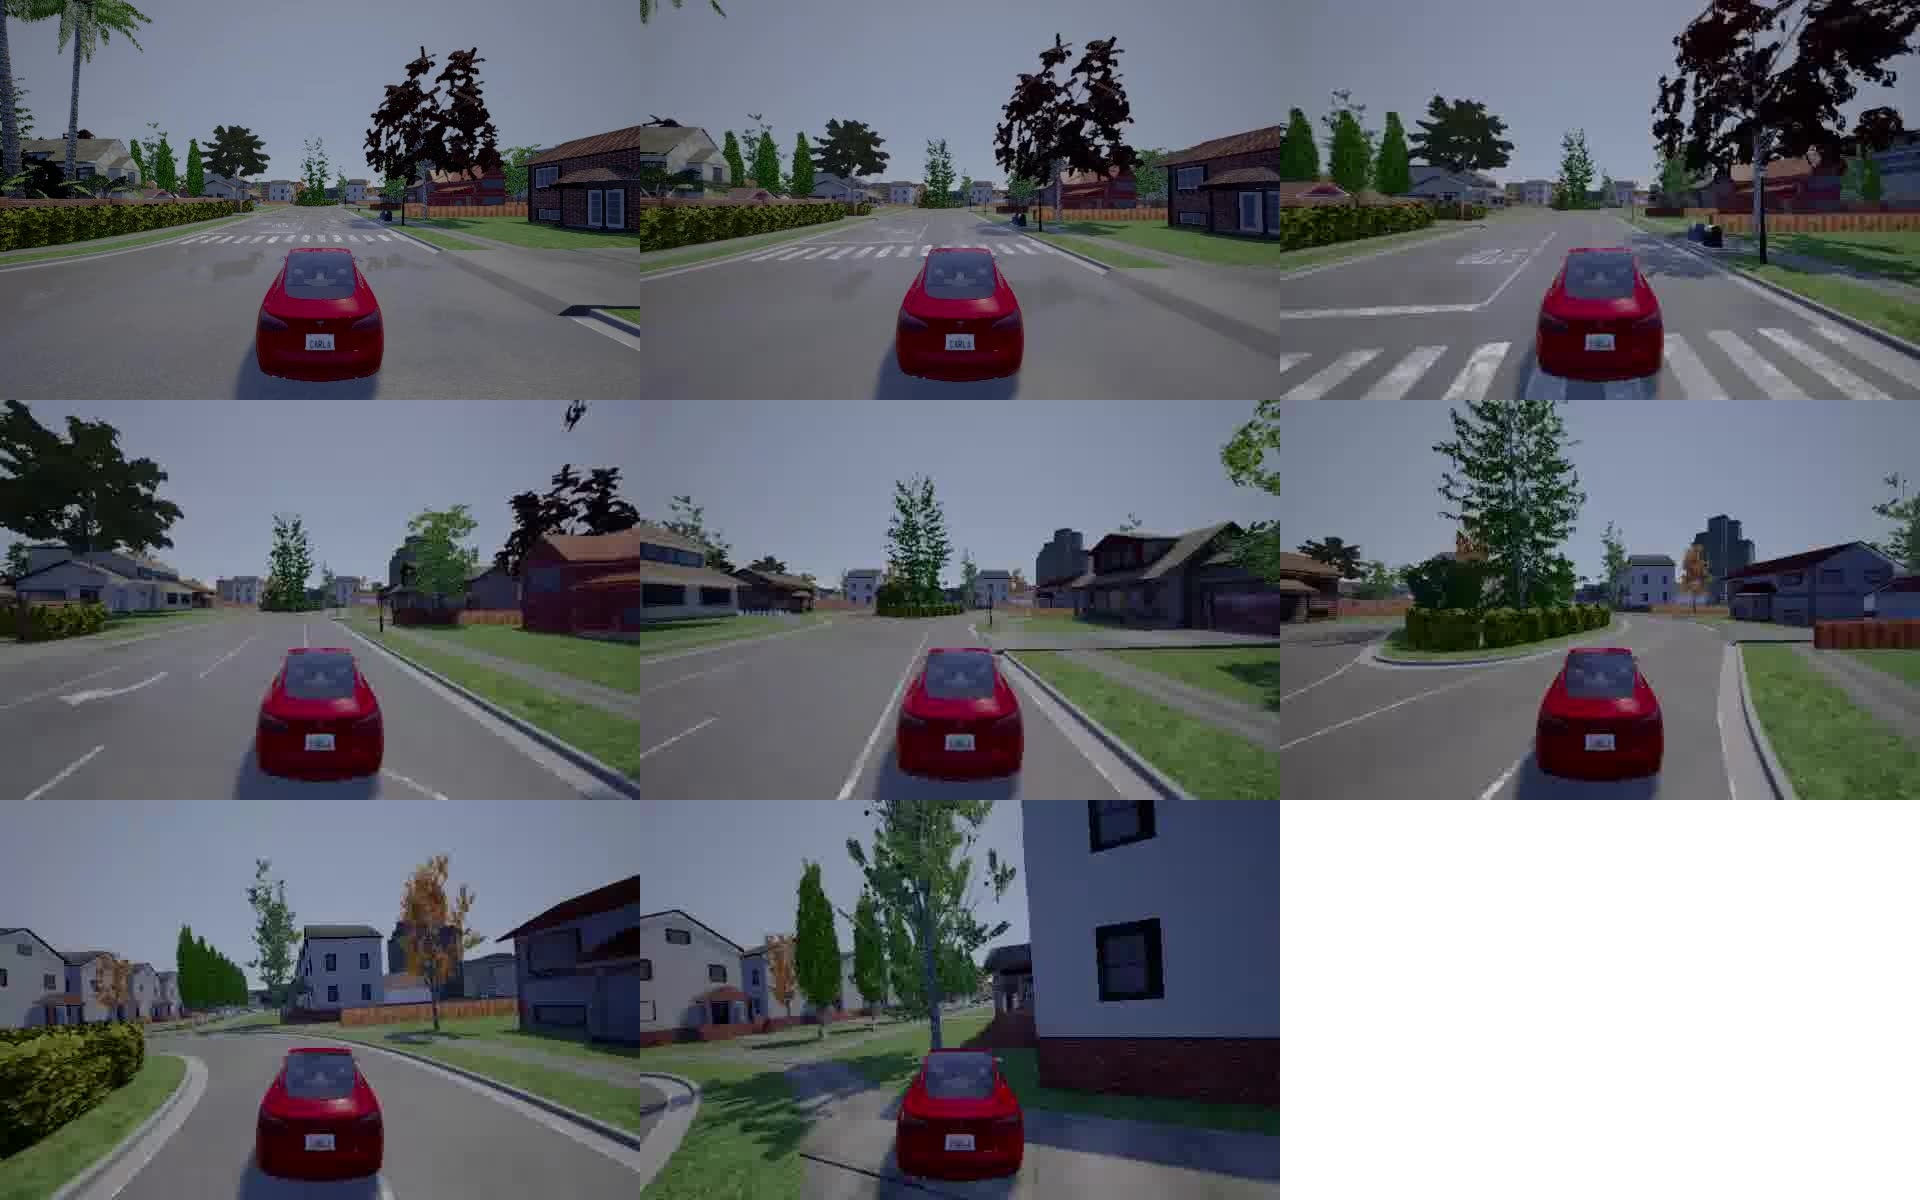
\includegraphics[width=1\linewidth]{images/uji0}
	\caption{Salah satu hasil simulasi uji. Jarak antar foto adalah 1.5 detik. Baca sekuen dari atas kiri ke kanan bawah.}
	\label{fig:uji0}
\end{figure}

\subsection{Hasil Setelah Learning 58 jam}
\label{sec:hasil_learning_12}
Setelah learning selama 58 jam, didapatkan model reinforcement yang sudah cukup memahami gerakan bahwa agent harus memutari bundaran agar mendapatkan award yang lebih besar. Pada salah satu run simulasi Gambar \ref{fig:uji1}., didapatkan agent yang mampu bergerak lurus ke depan hingga mendekati bundaran, dan mampu melakukan manuver kiri untuk menghindari bundaran, lalu melakukan manuver ke kanan mengitari bundaran dan tidak menyentuh bundaran. Meskipun pada akhirnya agent menyentuh object pagar setelah mengitari hampir 3/4 dari bundaran.
\begin{figure}[H] 
	\centering
	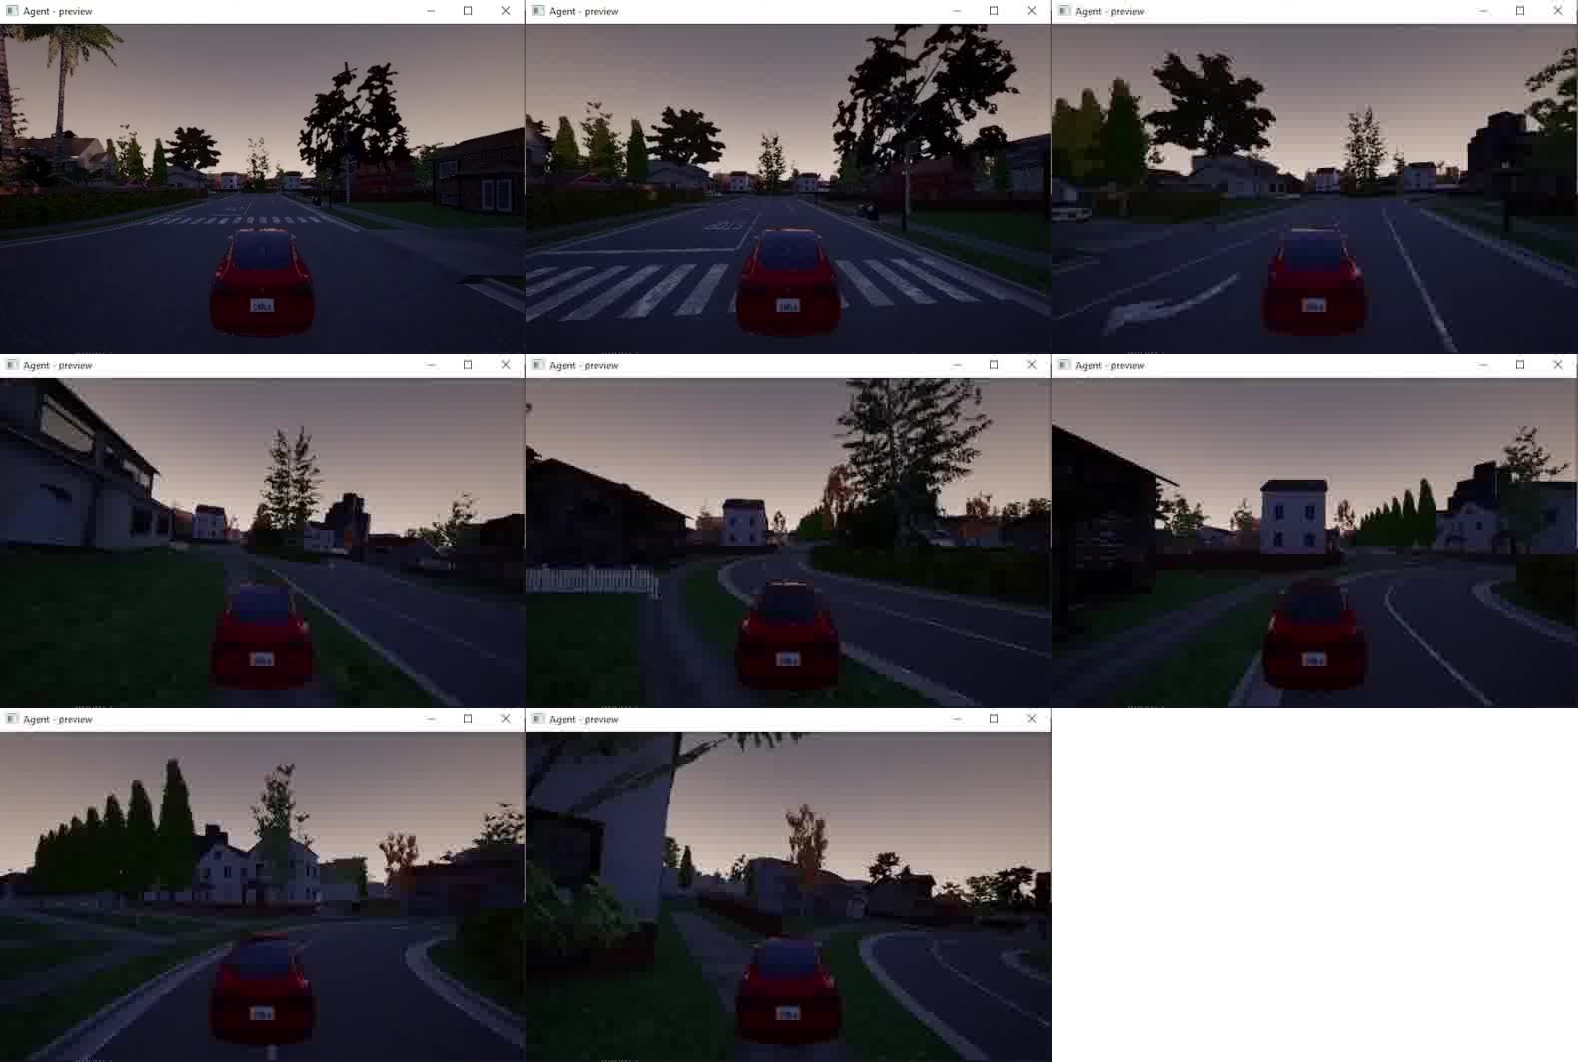
\includegraphics[width=1\linewidth]{images/uji1}
	\caption{Salah satu hasil simulasi uji. Jarak antar foto adalah 1.2 detik. Baca sekuen dari atas kiri ke kanan bawah.}
	\label{fig:uji1}
\end{figure}
\fi
